
%\DeclareMathOperator{\tri}{tri} \DeclareMathOperator{\rect}{rect}
%\DeclareMathOperator{\sgn}{sgn} \DeclareMathOperator{\ramp}{ramp}
%\DeclareMathOperator{\sinc}{sinc}


\subsection{Co\"ordinatenstelsels}

%\begin{itemize}
%\item Hoe kunnen we op een \'e\'enduidige manier elk punt in het vlak of de
%ruimte een plaats geven?
%\item Welke co\"ordinatenstelsels worden er vaak gebruikt?
%\end{itemize}
%Een co\"ordinatenstelsel is een wiskundige methode die wordt gebruikt
%om de ligging van een punt weer te geven.

\subsubsection{Cartesisch of rechthoekig co\"ordinatenstelsel}

De vergelijking $y=f(x)$ voegt aan iedere $x$-waarde \'e\'enduidig een
$y$-waarde toe. Met $x_{0}$ komt bijvoorbeeld $y_{0}$ overeen volgens
$y_{0}=f(x_{0})$. Het getallenpaar $(x_{0}\,,\,y_{0})$ kunnen we
als punt P in een rechthoekig of cartesisch co\"ordinatenstelsel tekenen.
De twee co\"ordinaat-assen staan loodrecht op elkaar, de horizontale
as noemen we de $x$-as en de verticale as de $y$-as. Het snijpunt is de
oorsprong O.

Voor ieder getallenpaar krijgen we precies \'e\'en punt. De
verzameling van alle punten $(x\,,\,y=f(x))$ vormt de grafiek of
kromme van de functie. De grafiek laat het verloop van de functie
in een figuur zien.

%\gewonefiguur{height=5cm}{2_elem_rekenvaardigheden_B/inputs/figuur10}

\begin{figure}[H]
\centering
\begin{center}
	\begin{tikzpicture}[yscale=2,cap=round]
	
	% Styles
	\tikzstyle{axes}=[]
	\tikzstyle help lines=[color=blue!50,very thin,dotted]
	
	% grid
%	\draw[style=help lines,step=1cm] (-4.9,-1.9) grid (4.9,4.9);
	
	\draw[->] (-1,0) -- (8,0) node[right] {$x$};
	\draw[->] (0,-.5) -- (0,2) node[above] {$y$};
	
	%\draw[fill,cyan](1,1)circle [radius=0.025];
	%FUNCTIEVOORSCHRIFTEN
	
	

	
	
	
	\draw[red,cap=rect,line width=1, opacity=1, domain=1:6,samples=100] plot (\x, {
	-1* exp(pow(0.5,\x))+2	% <- plaats het functievoorschrift hier	
	}) node[opacity=1,above,right]{$y=f(x)$};
	%-------------------------------------------
	
	
	\draw[dotted] (4,0)--(4,0.95); 
	\draw[dotted] (0,0.95)--(4,0.95); 
	
	\draw[] (4,0) node[below]{$x_0$};
	\draw[] (0,0.95) node[left]{$y_0$};
	
	\draw[] (4,1) node[above]{$P$};
	
	\draw[] (-0.2,0) node[left,below]{$0$};
	
	

	%legende
	
	
	
	%getallen op de x-as en lijntjes   
%	\foreach \x/\xtext in {-4,-3,-2,-1,0,1,2,3,4}
%	\draw[xshift=\x cm] (0pt,1pt) -- (0pt,0pt) node[below,fill=white]
%	{$\xtext$};,3
	
	%getallen op de y-as en lijntjes  
	%BEGIN LUS
%	\foreach \y/\ytext in {-1,1,2,3,4}
%	\draw[yshift=\y cm] (1pt,0pt) -- (0pt,0pt) node[left,fill=white]
%	{$\ytext$}; %EINDE LUS
	
	
	
	\end{tikzpicture}
\end{center}


\end{figure}


\begin{tabel*}{}
	\centering
\begin{tabular}{cll}
	We zeggen dat: & $x_{0},y_{0}$  & zijn de rechthoekige of cartesische co\"ordinaten\\
	& $x_{0}$  & is de abscis van het punt P\\
	& $y_{0}$ & is de ordinaat van het punt P\\
\end{tabular}
\end{tabel*}

Het cartesisch co\"ordinatenstelsel is de gebruikelijke manier
om een punt in een vlak aan te duiden. Omdat in dit platte vlak twee
co\"ordinaten nodig zijn om een punt vast te leggen, zeggen we dat een
vlak tweedimensionaal is. In feite is \textquoteleft de dimensie van een ruimte\textquoteright \
het aantal co\"ordinaten dat nodig is om de plaats van alle punten in
die ruimte precies te kunnen bepalen. Zo bestaat de klassieke 3D-ruimte
uit 3 dimensies en zijn er dus 3 co\"ordinaten $(x,y,z)$ nodig om de
plaats van elk punt \'e\'enduidig te beschrijven. 

\subsubsection{Parametervoorstelling van een functie}

Het is bij de wiskundige beschrijving van een bewegend lichaam
vaak handig om de positie van het lichaam weer te geven door cartesische
co\"ordinaten die zelf een functie van de tijd zijn. We noteren dan:

\begin{equation*}
x=x(t)\:,\;y=y(t)\quad\textrm{met}\:t_{1}\leq t\leq t_{2}
\end{equation*}

We noemen een dergelijke voorstelling met een hulpvariabele
$t$ de parametervoorstelling van een functie. In de natuurwetenschappen
en de techniek betekent de parameter $t$ meestal de tijd of een hoek.

We krijgen voor iedere waarde van $t$ uit het interval $t_{1}\leq t\leq t_{2}$
precies \'e\'en punt van de kromme.


\begin{voorbeeld}
	de horizontale worp

een lichaam wordt van een bepaalde hoogte horizontaal met
een constante beginsnelheid $v_{0}$ weggeworpen. T.g.v. de zwaartekracht
verloopt de beweging vervolgens als een parabool (parabolische baan).
De parametervergelijkingen van deze beweging zijn:

\begin{equation*}
x=v_{0}t\:,\;y=\frac{1}{2}gt^{2}\quad\textrm{met}\:t\geq0
\end{equation*}


Door het elimineren van de parameter vinden we de expliciete
vergelijking van de grafiek (parabool). Dit doen we door t uit de
vergelijking van $x$ te halen en te substitueren in de vergelijking
van $y$: uit $x=v_{0}t$ volgt dat $t=\frac{x}{v_{0}}$ zodat \begin{equation*}
y=\frac{1}{2}gt^{2}=\frac{1}{2}g\left(\frac{x}{v_{0}}\right)^{2}=\frac{g}{2v_{0}^{2}}x
\end{equation*}

\end{voorbeeld}

\begin{voorbeeld}
	de cirkel

Een veel gebruikte parametrisatie voor de cirkel met vergelijking
$x^{2}+y^{2}=R^{2}$ is de volgende:

\begin{equation*}
x=R\cos(t)\:,\;y=R\sin(t)\quad\textrm{met}\:0\leq t<2\pi
\end{equation*}

\begin{opmerking}
	\ \\
	\begin{itemize}
\item de parameter $t$ stelt nu een hoek voor (uitgedrukt in radialen).
Omdat $t=0$ en $t=2\pi$ hetzelfde punt voorstellen, zal men meestal
$2\pi$ niet opnemen in het interval. Vandaar het $<$ en niet nog
eens het $\leq$-symbool.
\item om uit de parametervergelijkingen de cartesische vergelijking voor
de cirkel te bekomen moeten we de parameter $t$ elimineren. Daarvoor
gebruiken we een trucje. We weten dat voor elke hoek $\alpha$ de
goniometrische grondformule geldt: $\cos^{2}\alpha+\sin^{2}\alpha=1$.
Substitueren we nu $\cos(t)=\frac{x}{R}$ en $\sin(t)=\frac{y}{R}$
in de grondformule dan bekomen we inderdaad $x^{2}+y^{2}=R^{2}$.
\end{itemize}

\end{opmerking}
\end{voorbeeld}


\subsubsection{Poolco\"ordinaten}

De poolco\"ordinaten $\left(r,\theta\right)$ van een punt $P$ in een
vlak zijn de afstandsco\"ordinaat $r$ en de hoekco\"ordinaat $\theta$.
We noemen de afstand $r$ de radius of de voerstraal en de hoek $\theta$
het argument.

%\begin{figure}
%\centering
%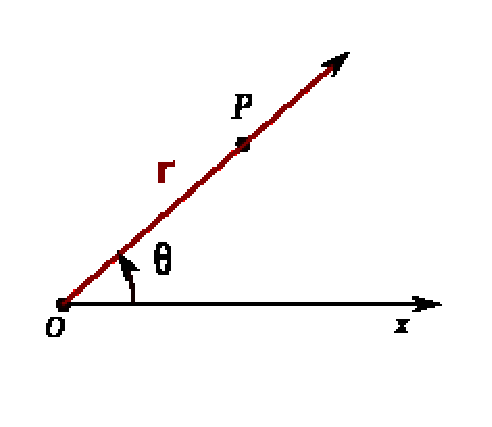
\includegraphics{2_elem_rekenvaardigheden_B/inputs/Poolcoordinaten_wikipedia}
%\end{figure}

\begin{center}
	\tikzsetfigurename{module2_1_16_poolcoordinaten}
\begin{tikzpicture}

\coordinate (a) at (0,0) node[anchor=south,below,xshift=-0.3cm]{$O$};
\coordinate (b) at (1,0);
\coordinate (c) at (2.5,3);

\draw[thin,gray!40] (-3,-1) (3,3);
\draw[->] (0,0)--(3,0) node[right]{$x$};
%\draw[->] (0,-1)--(0,3) node[above]{$y$};
%\draw[line width=2pt,black,-stealth](0,0)--(2,0) node[anchor=south,xshift=0.3cm]{$\vec{e_x}$};
%\draw[line width=2pt,black,-stealth](0,0)--(0,2) node[anchor=south,xshift=0.3cm]{$\vec{e_y}$};

%\draw[red] node[]{$P$}

%\draw[line width=2pt,blue,-stealth](0,0)--(1.732,1) node[anchor=south]{$\vec{e_u}$};
%\draw[line width=2pt,blue,-stealth](0,0)--(-1,1.732) node[anchor=south]{$\vec{e_v}$};

\draw[line width=1pt,red,-stealth](0,0)--(2.5,3) node[anchor=south,above, midway]{$r$} node[anchor=south]{$P$};

%\coordinate (d) at (2,2.4) node[anchor=south]{$P$}

%\path[clip] (0.866,0.5) -- (0,0) -- (0.866,0) -- cycle;
%\node[circle,draw=black,minimum size=40pt] at (0,0) (circ) {};
%\draw[blue] (1cm,0cm) arc (90:125:0.5cm);

%  \draw
%(3,-1) coordinate (a) node[right] {a}
%-- (0,0) coordinate (b) node[left] {b}
%-- (2,2) coordinate (c) node[above right] {c}
%pic["$\alpha$",draw=orange,<->,angle eccentricity=1.2,angle radius=1cm] {angle=a--b--c};

\pic [draw, ->, "$\theta$", angle eccentricity=1.5] {angle = b--a--c};


%\draw[line width=2pt,blue,-stealth](0,0)--(-0.5,$\sqrt{3}/2$) node[anchor=south]{$\vec{e_v}$};

\end{tikzpicture}
\end{center}

Enkele opmerkingen:
\begin{itemize}
\item we defini\"eren de voerstraal $r$ steeds positief, dus $r\geq0$.
\item we defini\"eren de hoek $\theta$ positief als de pijl van de positieve
$x$-as naar de plaatsvector van P tegen de klok in draait (andersom
is de hoek negatief). Een hoek $\theta$ is \'e\'enduidig bepaald op veelvouden
van 360\textdegree{} (of veelvouden van $2\pi$ in radialen) na. Meestal
wordt de hoek $\theta$ gegeven in het interval $0\text{\textdegree}\leq\theta\leq360\text{\textdegree}$
of $0\leq\theta\leq2\pi$. I.p.v. de Griekse letter theta ($\theta$) wordt ook vaak de letter phi ($\varphi$) als hoekaanduiding gebruikt.
\item de $x$- en $y$-as maken geen deel uit van dit co\"ordinatenstelsel. We tekenen
echter wel vaak een horizontale en verticale hulplijn om het uitzetten
van de hoeken te vergemakkelijken.
\item het poolco\"ordinatenstelsel is een kromlijnig co\"ordinatenstelsel: de
co\"ordinaatlijnen zijn concentrische cirkels met de oorsprong O als
middelpunt en langs stralen die radiaal vanuit O lopen. We noemen
de oorsprong ook vaak \textquoteleft de pool\textquoteright\ en de $x$-as de \textquoteleft poolas\textquoteright.
\item de pool (dus de oorsprong O) heeft als voerstraal $r=0$ terwijl de
hoek $\theta$ onbepaald is.
\item poolco\"ordinaten worden ook gebruikt bij het voorstellen van en het
werken met complexe getallen.
\end{itemize}

Soms is het handig of noodzakelijk om over te stappen van
cartesische co\"ordinaten naar poolco\"ordinaten of omgekeerd. Daarvoor
gebruiken we het volgende stel transformatievergelijkingen:

\vspace{1cm}

\begin{minipage}{.48\linewidth}
%\begin{table}
	\begin{tabular}{lcl}
		cartesische co\"ordinaten &  & poolco\"ordinaten  \\
		\hline
		gegeven P met $\left(x,y\right)$ & $\rightarrow$ & dan is $\begin{cases}
		r=\sqrt{x^{2}+y^{2}}\\
		\tan\theta=\frac{y}{x}
		\end{cases}$  \\
		dan is $\begin{cases}
		x=r\cdot\cos\theta\\
		y=r\cdot\sin\theta
		\end{cases}$ & $\leftarrow$ & gegeven P met $\left(r,\theta\right)$ \\
	\end{tabular}
%\end{table}
\end{minipage}
\hspace{1cm}
\begin{minipage}{.48\linewidth}
	\centering
%	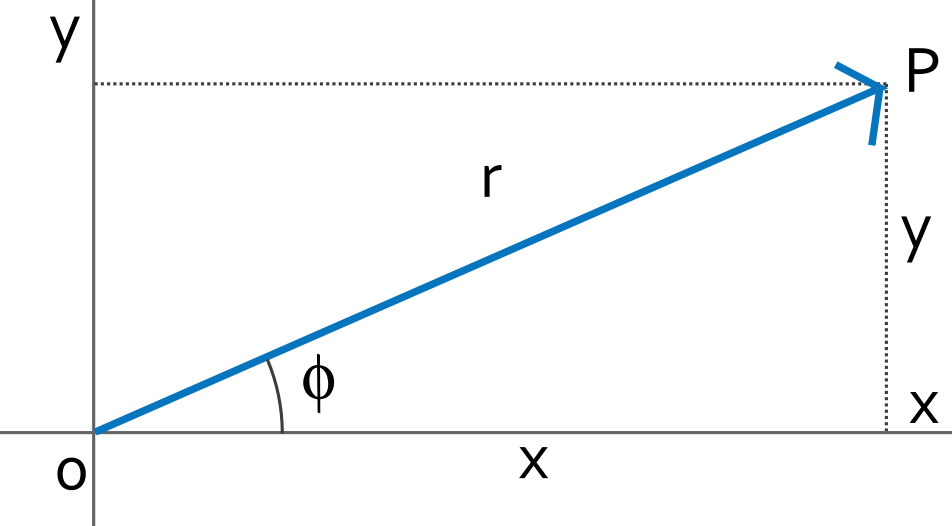
\includegraphics[width=0.7\linewidth]{2_elem_rekenvaardigheden_B/inputs/figuur9}
	\tikzsetfigurename{module2_1_16_poolcoordinaten2}
\begin{tikzpicture}

\coordinate (a) at (0,0) node[anchor=south,below,xshift=-0.3cm]{$O$};
\coordinate (b) at (1,0);
\coordinate (c) at (2.5,3);

\draw[thin,gray!40] (-3,-1) (3,3);
\draw[->] (-1,0)--(4,0) node[right]{$x$};
\draw[->] (0,-1)--(0,4) node[above]{$y$};
%\draw[line width=2pt,black,-stealth](0,0)--(2,0) node[anchor=south,xshift=0.3cm]{$\vec{e_x}$};
%\draw[line width=2pt,black,-stealth](0,0)--(0,2) node[anchor=south,xshift=0.3cm]{$\vec{e_y}$};

%\draw[red] node[]{$P$}

\draw[line width=0.5pt,dashed](2.5,0)--(2.5,3);
\draw[line width=0.5pt,dashed](0,3)--(2.5,3);

\draw[-] (0,0)--(2.5,0) node[anchor=south,below,midway]{$x$};
\draw[-] (0,0)--(0,3) node[anchor=south,left,midway]{$y$};

\draw[line width=1pt,-stealth](0,0)--(2.5,3) node[anchor=south,left,midway]{$r$} node[anchor=south]{$P$};

%\coordinate (d) at (2,2.4) node[anchor=south]{$P$}

%\path[clip] (0.866,0.5) -- (0,0) -- (0.866,0) -- cycle;
%\node[circle,draw=black,minimum size=40pt] at (0,0) (circ) {};
%\draw[blue] (1cm,0cm) arc (90:125:0.5cm);

%  \draw
%(3,-1) coordinate (a) node[right] {a}
%-- (0,0) coordinate (b) node[left] {b}
%-- (2,2) coordinate (c) node[above right] {c}
%pic["$\alpha$",draw=orange,<->,angle eccentricity=1.2,angle radius=1cm] {angle=a--b--c};

\pic [draw, ->, "$\theta$", angle eccentricity=1.5] {angle = b--a--c};


%\draw[line width=2pt,blue,-stealth](0,0)--(-0.5,$\sqrt{3}/2$) node[anchor=south]{$\vec{e_v}$};

\end{tikzpicture}
\end{minipage}

\vspace{1cm}

\begin{opmerking}
let op bij het berekenen van de hoek $\theta$. Je rekenmachine
zal als resultaat van de $\textrm{Arctan}\left(\frac{y}{x}\right)$
een hoek geven in het 1ste of 4de kwadrant. Je moet dus zelf, bij
het resultaat van je rekenmachine nog 180\textdegree{} of $\pi$ optellen
als het punt P in het 2de of 3de kwadrant ligt.
\end{opmerking}

De voorstelling van een functie in poolco\"ordinaten

Een functie (kromme) in poolco\"ordinaten wordt beschreven
door een vergelijking van de vorm: $r=r(\theta)$


We stellen een functiewaardentabel op voordat we de grafiek
van de functie tekenen. Voor verschillende waarden $\theta_{1}$ ,
$\theta_{2}$ , $\theta_{3}$ , ... berekenen we de bijhorende voerstralen
$r_{1}=r\left(\theta_{1}\right)$ , ... Daarna tekenen we de punten
met co\"ordinaten $\left(r_{1},\theta_{1}\right)$ , ... en verbinden
deze d.m.v. een vloeiende lijn.

\begin{minipage}{.48\linewidth}
	\centering
	\begin{tabular}{c|c}
		$\theta$ & $r=r(\theta)$\\
		\hline 
		$\theta_{1}$ & $r_{1}=r\left(\theta_{1}\right)$ \\
		$\theta_{2}$ & $r_{2}=r\left(\theta_{2}\right)$ \\
		$\vdots$ & $\vdots$\\
	\end{tabular}
\end{minipage}
\begin{minipage}{.48\linewidth}
%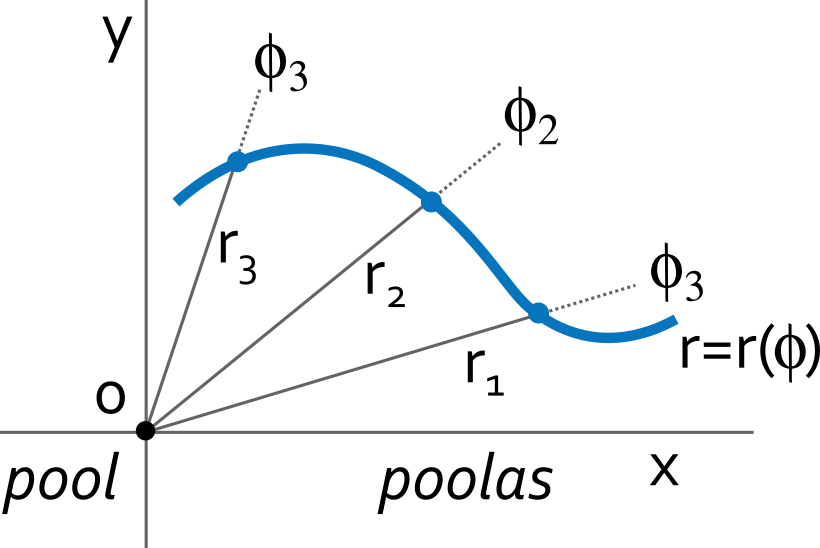
\includegraphics[height=5cm]{2_elem_rekenvaardigheden_B/inputs/figuur11}\\
%In de figuur zijn de hoeken aangeduid met $\phi$ i.p.v. $\theta$
\tikzsetfigurename{module2_1_16_poolcoordinaten3}
\begin{tikzpicture}

\coordinate (a) at (0,0) node[anchor=south,below,xshift=-0.3cm]{$O$};
\coordinate (a) at (0,0) node[anchor=south,below,xshift=-0.5cm,yshift=-0.5cm]{Pool};
\coordinate (b) at (1,0);
\coordinate (c) at (2.5,3);

\draw[thin,gray!40] (-3,-1) (3,3);
\draw[->] (-1,0)--(4,0) node[right]{$x$};
\draw[->] (0,-1)--(0,4) node[above]{$y$};
%\draw[line width=2pt,black,-stealth](0,0)--(2,0) node[anchor=south,xshift=0.3cm]{$\vec{e_x}$};
%\draw[line width=2pt,black,-stealth](0,0)--(0,2) node[anchor=south,xshift=0.3cm]{$\vec{e_y}$};


\draw[-] (0,0)--(2.5,0) node[anchor=south,below,midway]{Poolas};

\draw[line width=1pt](0,0)--(1,3) node[anchor=south,left,midway]{$r_3$};
\draw[dotted] (1,3)--(1.5,4.5) node[anchor=north,left]{$\theta_{3}$};
\draw[line width=1pt](0,0)--(1.5,1.5) node[anchor=south,left,midway]{$r_2$};
 \draw[dotted] (1.5,1.5)--(2,2) node[anchor=north,left]{$\theta_{2}$};
\draw[line width=1pt](0,0)--(3,1) node[anchor=south,left,midway]{$r_1$};
 \draw[dotted] (3,1)--(4,4/3) node[anchor=north]{$\theta_{1}$};

\draw[teal,cap=rect,line width=1, opacity=1, domain=0.7:3.5] plot (\x, {
	4/3*pow(\x,2)-19/3*pow(\x,1)+8  		% <- plaats het functievoorschrift hier
}) node[right,opacity=1]{$r=r(\theta)$};

%\coordinate (d) at (2,2.4) node[anchor=south]{$P$}

%\path[clip] (0.866,0.5) -- (0,0) -- (0.866,0) -- cycle;
%\node[circle,draw=black,minimum size=40pt] at (0,0) (circ) {};
%\draw[blue] (1cm,0cm) arc (90:125:0.5cm);

%  \draw
%(3,-1) coordinate (a) node[right] {a}
%-- (0,0) coordinate (b) node[left] {b}
%-- (2,2) coordinate (c) node[above right] {c}
%pic["$\alpha$",draw=orange,<->,angle eccentricity=1.2,angle radius=1cm] {angle=a--b--c};

%\pic [draw, ->, "$\theta$", angle eccentricity=1.5] {angle = b--a--c};


%\draw[line width=2pt,blue,-stealth](0,0)--(-0.5,$\sqrt{3}/2$) node[anchor=south]{$\vec{e_v}$};

\end{tikzpicture}
\end{minipage}



\begin{voorbeeld}
	de spiraal van Archimedes

Schets de kromme met vergelijking $r=\theta$ waarbij $0\leq\theta\leq2\pi$

We stellen een functiewaardentabel op (tip: kies niet te veel, maar
ook niet te weinig hoeken; de intervallen tussen de hoeken hoeft niet
noodzakelijk overal even groot te zijn).

\begin{minipage}{.48\linewidth}
	\centering
	\begin{tabular}{c|c}
		$\theta$ & $r=r(\theta)=\theta$\\
		\hline 
		$0$ & 0\\
		$\frac{\pi}{4}$ & 0,785 \\
		$\frac{\pi}{2}$ & 1,571\\
		$3\frac{\pi}{4}$ & 2,356\\
		$\pi$ & 3,142\\
		$3\frac{\pi}{2}$ & 4,712\\
		$2\pi$ & 6,283\\
	\end{tabular}
\end{minipage}
\begin{minipage}{.48\linewidth}
%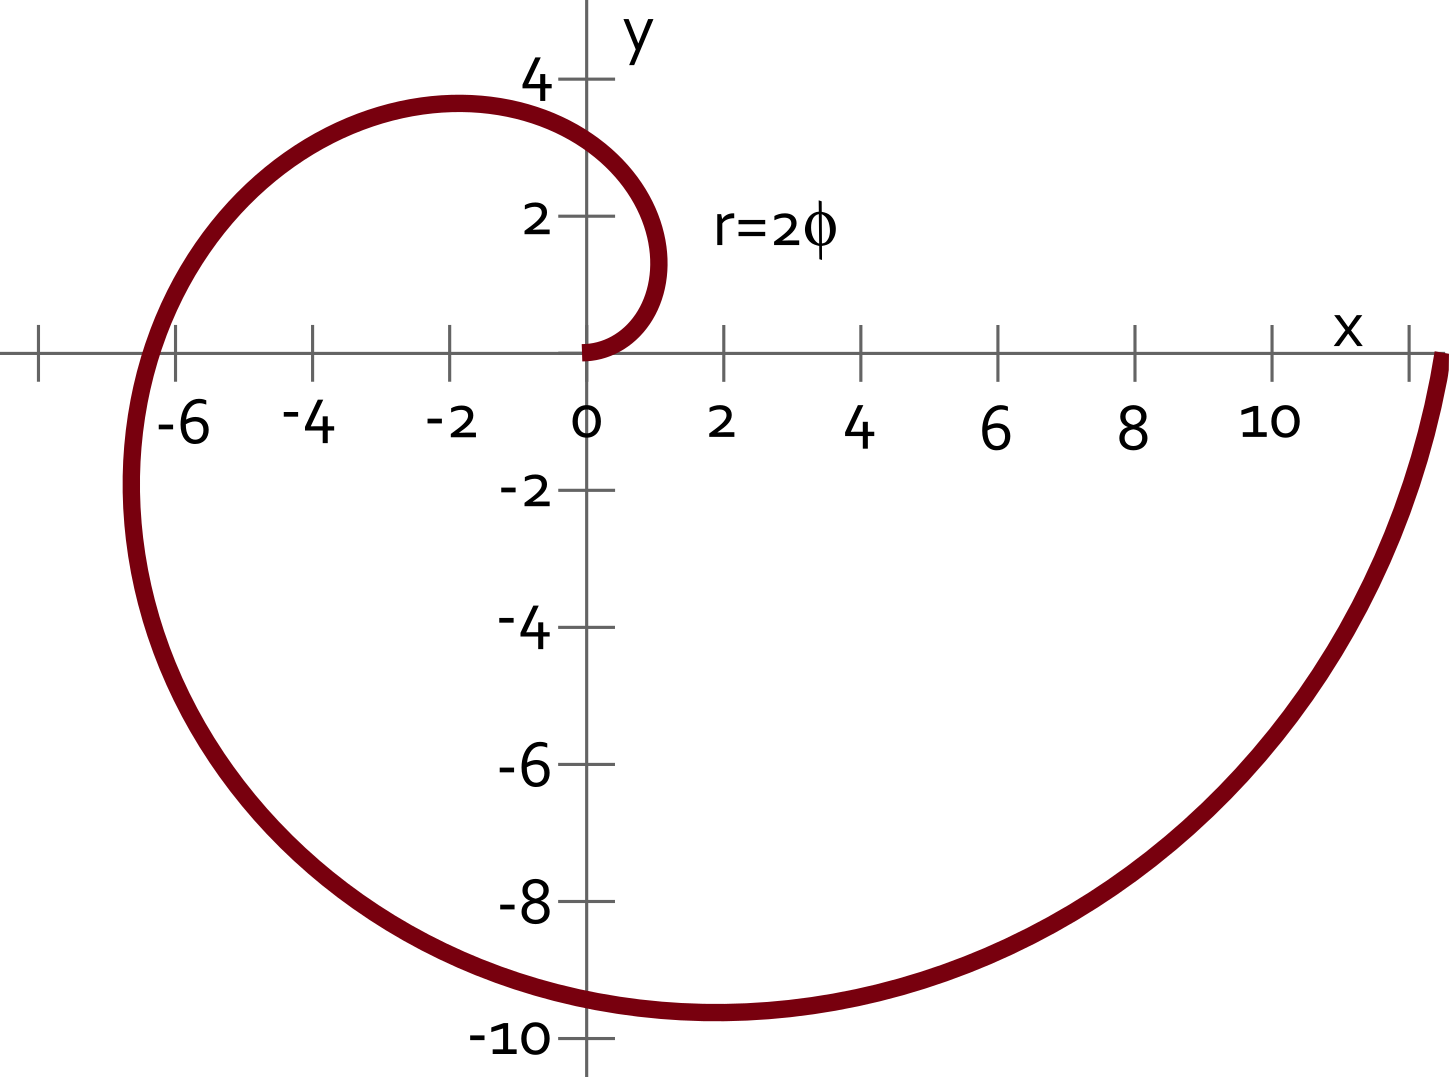
\includegraphics[height=5cm]{2_elem_rekenvaardigheden_B/inputs/figuur8}
\tikzsetfigurename{module2_1_16_poolcoordinaten4}
\begin{tikzpicture}[scale=0.6,cap=round]

% Styles
\tikzstyle{axes}=[]
\tikzstyle help lines=[color=black,very thin,dotted]

% grid
\draw[style=help lines,step=1cm] (-4,-5) grid (8,2);

\coordinate (a) at (0,0) node[anchor=south,below,xshift=-0.3cm]{$O$};
%\coordinate (a) at (0,0) node[anchor=south,below,xshift=-0.5cm,yshift=-0.5cm]{Pool};
\coordinate (b) at (1,0);
\coordinate (c) at (2.5,3);

\draw[thin,gray!40] (-3,-1) (3,3);
\draw[->] (-4,0)--(8,0) node[right]{$x$};
\draw[->] (0,-5)--(0,2) node[above]{$y$};
%\draw[line width=2pt,black,-stealth](0,0)--(2,0) node[anchor=south,xshift=0.3cm]{$\vec{e_x}$};
%\draw[line width=2pt,black,-stealth](0,0)--(0,2) node[anchor=south,xshift=0.3cm]{$\vec{e_y}$};


%\draw[-] (0,0)--(2.5,0) node[anchor=south,below,midway]{Poolas};

%\draw[line width=1pt](0,0)--(1,3) node[anchor=south,left,midway]{$r_3$};
%\draw[dotted] (1,3)--(1.5,4.5) node[anchor=north,left]{$\theta_{3}$};
%\draw[line width=1pt](0,0)--(1.5,1.5) node[anchor=south,left,midway]{$r_2$};
% \draw[dotted] (1.5,1.5)--(2,2) node[anchor=north,left]{$\theta_{2}$};
%\draw[line width=1pt](0,0)--(3,1) node[anchor=south,left,midway]{$r_1$};
% \draw[dotted] (3,1)--(4,4/3) node[anchor=north]{$\theta_{1}$};

%\draw[teal,cap=rect,line width=1, opacity=1, domain=0:2*pi] plot(({deg(\x)}:{cos(\x/3 r)^3}) 		% <- plaats het functievoorschrift hier
%}) node[right,opacity=1]{$r=r(\theta)$};

\draw [thick, color=red, domain=0:2*pi, samples=200, smooth]
plot (xy polar cs:angle=\x r, radius={\x}) node[right,above,opacity=1]{$r=\theta$};


%\coordinate (d) at (2,2.4) node[anchor=south]{$P$}

%\path[clip] (0.866,0.5) -- (0,0) -- (0.866,0) -- cycle;
%\node[circle,draw=black,minimum size=40pt] at (0,0) (circ) {};
%\draw[blue] (1cm,0cm) arc (90:125:0.5cm);

%  \draw
%(3,-1) coordinate (a) node[right] {a}
%-- (0,0) coordinate (b) node[left] {b}
%-- (2,2) coordinate (c) node[above right] {c}
%pic["$\alpha$",draw=orange,<->,angle eccentricity=1.2,angle radius=1cm] {angle=a--b--c};

%\pic [draw, ->, "$\theta$", angle eccentricity=1.5] {angle = b--a--c};


%\draw[line width=2pt,blue,-stealth](0,0)--(-0.5,$\sqrt{3}/2$) node[anchor=south]{$\vec{e_v}$};

\end{tikzpicture}
\end{minipage}

\end{voorbeeld}
\begin{voorbeeld}
	de cardio\"ide

Schets de kromme met vergelijking $r=1+\cos\theta$ waarbij $0\text{\textdegree}\leq\theta\leq360\text{\textdegree}$

We stellen een functiewaardentabel op. Wegens de symmetrie t.o.v.
de $x$-as berekenen we slechts de radius-waarden tussen 0\textdegree{}
en 180\textdegree .

\begin{minipage}{0.5\linewidth}
	\centering
\begin{tabular}{c|c}
$\theta$ & $r=r(\theta)$\\
\hline 
0\textdegree{} & 2\\
30\textdegree{} & 1,866\\
60\textdegree{} & 1,5\\
90\textdegree{} & 1\\
120\textdegree{} & 0,5\\
150\textdegree{} & 0,134\\
180\textdegree{} & 0\\
\end{tabular}
\end{minipage}
\begin{minipage}{.48\linewidth}
%	\begin{figure}
%	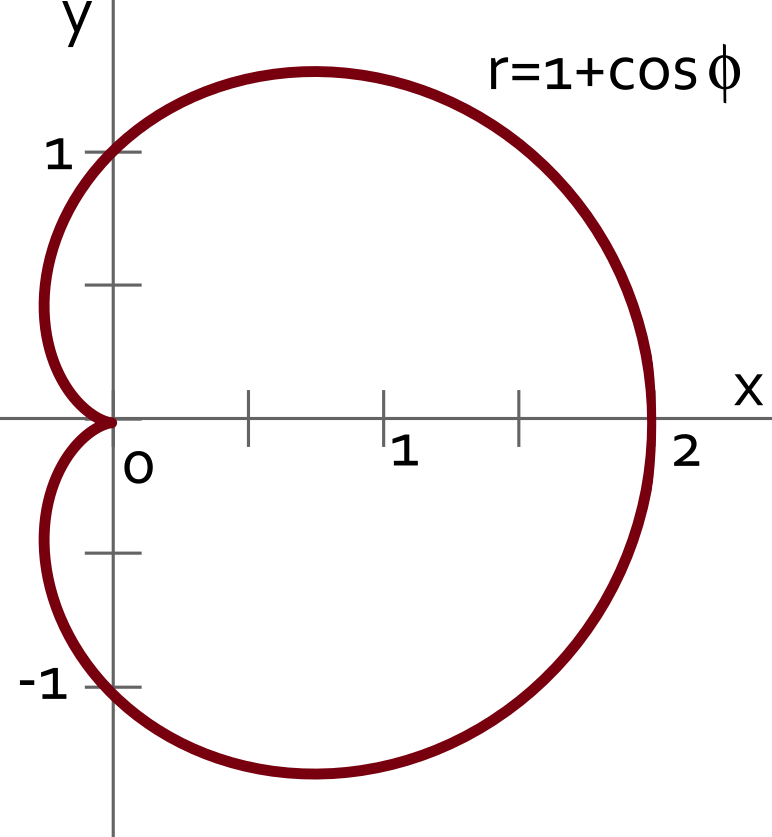
\includegraphics[height=5cm]{2_elem_rekenvaardigheden_B/inputs/figuur7.png}
	\tikzsetfigurename{module2_1_16_poolcoordinaten5}
\begin{tikzpicture}[cap=round]

% Styles
\tikzstyle{axes}=[]
\tikzstyle help lines=[color=black,very thin,dotted]

% grid
\draw[style=help lines,step=1cm] (-1,-2) grid (3,2);

\coordinate (a) at (0,0) node[anchor=south,below,xshift=-0.3cm]{$O$};
%\coordinate (a) at (0,0) node[anchor=south,below,xshift=-0.5cm,yshift=-0.5cm]{Pool};
\coordinate (b) at (1,0);
\coordinate (c) at (2.5,3);

\draw[thin,gray!40] (-3,-1) (3,3);
\draw[->] (-1,0)--(3,0) node[right]{$x$};
\draw[->] (0,-2)--(0,2) node[above]{$y$};
%\draw[line width=2pt,black,-stealth](0,0)--(2,0) node[anchor=south,xshift=0.3cm]{$\vec{e_x}$};
%\draw[line width=2pt,black,-stealth](0,0)--(0,2) node[anchor=south,xshift=0.3cm]{$\vec{e_y}$};


%\draw[-] (0,0)--(2.5,0) node[anchor=south,below,midway]{Poolas};

%\draw[line width=1pt](0,0)--(1,3) node[anchor=south,left,midway]{$r_3$};
%\draw[dotted] (1,3)--(1.5,4.5) node[anchor=north,left]{$\theta_{3}$};
%\draw[line width=1pt](0,0)--(1.5,1.5) node[anchor=south,left,midway]{$r_2$};
% \draw[dotted] (1.5,1.5)--(2,2) node[anchor=north,left]{$\theta_{2}$};
%\draw[line width=1pt](0,0)--(3,1) node[anchor=south,left,midway]{$r_1$};
% \draw[dotted] (3,1)--(4,4/3) node[anchor=north]{$\theta_{1}$};

%\draw[teal,cap=rect,line width=1, opacity=1, domain=0:2*pi] plot(({deg(\x)}:{cos(\x/3 r)^3}) 		% <- plaats het functievoorschrift hier
%}) node[right,opacity=1]{$r=r(\theta)$};

\draw [thick, color=red, domain=0:2*pi, samples=200, smooth]
plot (xy polar cs:angle=\x r, radius={1+cos(\x r)});
\node at (2,1.7) {$r=1+\cos(\theta)$};

%\coordinate (d) at (2,2.4) node[anchor=south]{$P$}

%\path[clip] (0.866,0.5) -- (0,0) -- (0.866,0) -- cycle;
%\node[circle,draw=black,minimum size=40pt] at (0,0) (circ) {};
%\draw[blue] (1cm,0cm) arc (90:125:0.5cm);

%  \draw
%(3,-1) coordinate (a) node[right] {a}
%-- (0,0) coordinate (b) node[left] {b}
%-- (2,2) coordinate (c) node[above right] {c}
%pic["$\alpha$",draw=orange,<->,angle eccentricity=1.2,angle radius=1cm] {angle=a--b--c};

%\pic [draw, ->, "$\theta$", angle eccentricity=1.5] {angle = b--a--c};


%\draw[line width=2pt,blue,-stealth](0,0)--(-0.5,$\sqrt{3}/2$) node[anchor=south]{$\vec{e_v}$};

\end{tikzpicture}
%	\end{figure}
\end{minipage} 

\end{voorbeeld}

\begin{voorbeeld}
	de cirkel

Schets de kromme met vergelijking $r=2$ waarbij $0\text{\textdegree}\leq\theta<360\text{\textdegree}$

Bij elke hoek $\theta$ hoort dezelfde voerstraal, namelijk $r=2$.
Het heeft dus weinig zin om een functiewaardentabel op te stellen.

Opmerking: de cartesische vergelijking van een cirkel heeft een duidelijk
ingewikkeldere notatie: $x^{2}+y^{2}=2^{2}$. Schrijven we $y$ expliciet
dan zien we meteen ook dat dit eigenlijk geen functie is (met elke
$x$-waarde komen immers 2 $y$-waarden overeen): $y=\pm\sqrt{4-x^{2}}$

\end{voorbeeld}